% =======================================================================
% =                                                                     =
% = ABNTEX - UTP                                                        =
% =                                                                     =
% =======================================================================
% -----------------------------------------------------------------------
% Author de configuração das normas : Chaua Queirolo
% Data:   01/07/2017
% -----------------------------------------------------------------------
% Author: Gabriel Pinto Ribeiro da Fonseca
% Data: 10/08/2019
% -----------------------------------------------------------------------
\documentclass[12pt,oneside,a4paper,chapter=TITLE,section=TITLE,sumario=tradicional]{abntex2}
% Regras da abnt
\usepackage{packages/abnt-UTP}
\usepackage{lipsum}
\usepackage{float}
\usepackage{longtable}

% =======================================================================
% =                                                                     =
% = DADOS DO TRABALHO                                                   =
% =                                                                     =
% =======================================================================

% Informações de dados para CAPA e FOLHA DE ROSTO
\titulo{Interpretador da linguagem D+}

\autor{Gabriel Pinto Ribeiro da Fonseca}

\orientador{Prof. Diógenes Cogo Furlan}

\preambulo{Trabalho de Conclusão de Curso apresentado ao curso de Bacharelado 
em Ciência da Computação da Faculdade de Ciências Exatas e de Tecnologia da 
Universidade Tuiuti do Paraná, como requisito à obtenção ao grau de Bacharel.}

\instituicao{Universidade Tuiuti do Paraná}
\local{Curitiba}
\data{2019}

% =======================================================================
% =                                                                     =
% = DOCUMENTO                                                           =
% =                                                                     =
% =======================================================================
\begin{document}

% -----------------------------------------------------------------------
% -                                                                     -
% - ELEMENTOS PRÉ-TEXTUAIS                                              -
% -                                                                     -
% -----------------------------------------------------------------------

% Capa e folha de rosto
\imprimircapa
\imprimirfolhaderosto

% Resumo
\begin{comment}
\begin{resumo}
    Texto do resumo.
    
    \palavraschave{Palavra 1, Palavra 2, Palavra 3}    
\end{resumo}
\end{comment}
% Listas
\listadefiguras

\listadegraficos
%\listadetabelas
\listadequadros
%\listadecodigos
%\listadealgoritmos
\begin{comment}
% Lista de siglas
\begin{siglas}
  \item[ABNT] Associação Brasileira de Normas Técnicas
\end{siglas}
% ---
\end{comment}
% Lista de símbolos
%\begin{simbolos}
 % \item[$ \Gamma $] Letra grega Gama
%  \item[$ \Lambda $] Lambda
%  \item[$ \zeta $] Letra grega minúscula zeta
%  \item[$ \in $] Pertence
%\end{simbolos}

% Sumario
\sumario

% -----------------------------------------------------------------------
% -                                                                     -
% - ELEMENTOS TEXTUAIS                                                  -
% -                                                                     -
% -----------------------------------------------------------------------
% Inicia a numeracao das páginas
\textual

% -----------------------------------------------------------------------
% -----------------------------------------------------------------------
\chapter{Introdução}
\label{cap:introducao}


Dentro do curso de bacharelado em ciências da computação, a disciplina de compiladores é responsável por apresentar ao aluno a forma e os significados contidos na construção de um compilador. Um compilador da forma convencional apresenta fases, análises, em que efetua os processos necessários para transformar o código da linguagem de alto nível para código de máquina. A disciplina de compiladores apresenta uma considerável dificuldade no seu aprendizado, uma vez que é uma disciplina muito abrangente e muito profunda. Ela faz uma síntese de todo curso de bacharelado em ciências da computação, uma vez que exige conhecimentos em algoritmos, programação estruturada e orientado a objetos, estrutura de dados, métodos de autômatos, gramáticas e ainda conhecimento de assembly. 

O presente projeto tem como objetivo o desenvolvimento de um interpretador da linguagem D+, para auxiliar os alunos na absorção do conteúdo, ajudando-os a fixar melhor os conceitos. O interpretador compila linha por linha e mostra visualmente em uma interface o programa já compilado. Neste software vai aplicar conteúdos visto em sala de aula, na prática, proporcionando ao aluno entender como eles são elaborados dentro dos processos de análise léxica e sintática.

Para desenvolver este software, é implementado um compilador D+, linguagem elaborada pelo mestre Diógenes Cogo Furlan. Este compilador terá modificações para se tornar um interpretador. Para o desenvolvimento deste software, é utilizado o editor QT Creator com a linguagem C++, pelo fato de que este editor juntamente com a linguagem, disponibiliza ferramentas que facilitam a sua criação.

Com este projeto, os alunos da disciplina de compiladores, terão ao seu alcance uma ferramenta (software) que os auxiliará no aprendizado da disciplina. Podendo criar códigos, e ver a transformação que passa pelo compilador, passando pela análise léxica, análise sintática e análise semântica. Os alunos que utilizarem este software, terão exemplos de árvores sintáticas no código escrito na interface. Com toda a informação apresentada para os estudantes da disciplina, é facilitado a compreensão da lógica de compiladores.

% -----------------------------------------------------------------------
% -----------------------------------------------------------------------
%\chapter{Fundamentação Teórica}
\chapter{Teoria da Compilação}
\label{cap:teoria-da-compilação}

Este capítulo tem como objetivo apresentar os conceitos envolvendo a compilação, técnicas encontradas nela, razão pelo qual foi criado, seu funcionamento e sua estrutura, como análise léxica, análise sintática e analise semântica, também explicando o funcionamento de um compilador e um interpretador, dando ênfase em suas diferenças.

Um processo de compilação designa o conjunto de tarefas que o compilador deve realizar para poder gerar uma descrição em uma linguagem a partir de outra \cite{pedro2018}. No começo da compilação, o compilador deve garantir que a tradução efetuada do código inserido seja correta, para que a execução dos comandos seja feita sem nenhum erro.

O motivo que influenciou o desenvolvimento dos compiladores se deve ao fato de se obter uma maior eficiência de programação. No princípio os computadores possuíam arquiteturas distintas entre eles, tornando assim a mesma instrução diferente para todas. Este mesmo problema era encontrado na representação de dados \cite{ricarte2008}.

Na figura 1 é ilustrado uma situação em que se utiliza uma instrução de soma, nesta imagem pode se observar a complexidade que a comunicação atingia ao transmitir para outra máquina a instrução. Devido a este empecilho, era necessária uma intervenção humana, ocasionando em contratar um especialista para resolver este problema, para cada plataforma. Uma situação pouco eficiente e de alto custo para a empresas  \cite{ricarte2008}.

\begin{figure}[htb]
    \legenda[fig:figura]{A programação antes dos compiladores}
    \fig{scale=1.0}{imagens/figura1}
    \fonte{\cite{ricarte2008}}
\end{figure}
RESOLVER
Para solucionar este problema, em busca de uma solução automática, procurando traduzir as especificações genéricas  RESOLVER \cite{ricarte2008}. Com este objetivo desenvolveu os compiladores.

A figura 2 ilustra o processo já incluindo os compiladores. Com essa automação na tradução do código, se obteve economia pelo fato de não ser necessário a contratação de um especialista para esta tarefa, e aumento de produtividade por ter retirado a intervenção humana em uma parte do processo. 

\begin{figure}[htb]
    \legenda[fig:figura]{A programação com compiladores}
    \fig{scale=1.0}{imagens/figura2}
    \fonte{\cite{ricarte2008}}
\end{figure}

\section{Compiladores}
\label{sec:compiladores}

Para se conceituar um compilador de forma simples, o compilador é um programa responsável por traduzir outro programa de uma linguagem fonte para outra linguagem alvo \cite{alfred1995}. Na figura 3 é demonstrado a forma do funcionamento dos compiladores como descrito acima, ilustrando os passos internos de um compilador, e o que é gerado em cada passo, como os tokens na análise léxica, árvore sintática na análise sintática e a tabela de símbolos.

\begin{figure}[htb]
    \legenda[fig:figura]{Exemplo do Funcionamento de um Compilador}
    \fig{scale=0.7}{imagens/figura3}
    \fonte{O próprio autor}
\end{figure}

O compilador segue passos para a tradução correta do código fonte para o código de saída. Os passos de análises são: análise léxica (AL), análise sintática (AS) e análise semântica (ASE). Os passos de tradução, são a Geração de código intermediário, a otimização de código, a geração de código final e a otimização de código final. Na figura 4 é ilustrado os passos seguidos dentro de um compilador, quando um código entra em seu processo, e é finalizado como o código de máquina alvo.

\begin{figure}[htb]
    \legenda[fig:figura]{Exemplo dos passos presentes em um compilador}
    \fig{scale=0.8}{imagens/figura5}
    \fonte{\cite{maragon2015}}
\end{figure}


\section{Interpretadores}
\label{sec:interpretadores}

O interpretador é o programa que converte a linguagem atual para uma especifica, mas ao contrário do compilador, ele não converte o código todo para linguagem de máquina de uma vez. Ele executa diretamente cada instrução, passo a passo. MATLAB, LISP, Perl e PHP são apontadas como interpretadas \cite{penelope2019}.  O interpretador efetua a tradução em operações especificadas, dependendo de como foi construído, podendo percorrer o código e ao decorrer desta análise, efetuar as operações necessárias. 

Na figura 5 é ilustrado um fluxo geral de como é convertido o código, comparando o compilador ao interpretador. O que difere entre ambos é em qual momento ocorre a inserção de dados, tempo de execução e a diferença na saída de arquivos após os processos, o compilador gera um arquivo com a linguagem alvo (neste caso linguagem de máquina), e o interpretador executa diretamente a instrução, sem criar um arquivo fonte.

\begin{figure}[htb]
    \legenda[fig:figura]{Comparação Compilador x Interpretador}
    \fig{scale=0.8}{imagens/figura4}
    \fonte{O próprio autor}
\end{figure}

Caso o código seja executado uma segunda vez, ocorrerá uma nova tradução, pois a tradução ocorrida anteriormente não fica armazenada para futuras execuções. Compiladores e interpretadores utilizam as análises léxica, análise sintática e análise semântica.

\section{Análise Léxica}
\label{sec:analise-lexica}

A análise Léxica, também chamada de análise \textit{scanning}, é responsável por analisar os caracteres no programa da esquerda para a direita, e agrupa-los para a formação de tokens. Tokens são sequencias de caracteres que possuem um significado coletivo \cite{alfred1995}.

Um exemplo que pode ser dado, é analisando um programa na linguagem C como ilustrado na figura 6.

\begin{figure}[htb]
    \legenda[fig:figura]{Código de exemplo para Análise Léxica}
    \fig{scale=1.0}{imagens/figura6}
    \fonte{O próprio autor}
\end{figure}

Efetuando uma análise léxica no código da linguagem C++ ilustrado na figura 6, é possível apontar os tokens criados e os erros encontrados neste passo. 

Descrevendo as linhas corretas e os tokens retirados dela.

\begin{lista}
	\item Identificador    X 
	\item Atribuição        = 
	\item Número            6 
	\item Identificador    Y
\end{lista}

Estes tokens citados acima, são os gerados na análise léxica, atribuídos e guardados para a próxima análise. Porém o código da figura 6 contém erros, impedindo de avançar para o próximo etapa.

Os erros encontrados na análise léxica são:

\begin{lista}
	\item Linha 8, o analisador léxico não conhece o caractere (\#) como algo valido;
	\item Linha 9, 15x não é reconhecido como número e nem como um identificador;
	\item Linha 11, é iniciado um comando de bloco de comentário (/*), mas não é fechado com (*/).
\end{lista}

Na figura 5 ocorrem erros de análise sintática, que é o passo que abordaremos no capítulo 2.4.

\subsection{Autômatos}
\label{sec:automatos}

Os autômatos finitos são conjuntos de estados e por transições dirigidas e rotuladas entre esses estados \cite{pedro2018}. Estes autômatos ilustram a expressão regular da gramática, e é através de seus passos que são verificados se uma cadeia de caracteres X faz parte da linguagem analisada ou não \cite{alfred1995}.

RESOLVER
Na figura 7 é ilustrado um autômato finito, cada estado é apresentado como uma esfera, as ligações entre elas são as validações, este autômato valida uma sequência de palavra "ABA", caso não seja essa a entrada e retornado erro. A primeira esfera possui um triangulo virado 90º para indicar que este é o início do autômato, e a última com uma esfera dentro para informar seu fim.RESOLVER

\begin{figure}[htb]
    \legenda[fig:figura]{Autômato Finito}
    \fig{scale=0.8}{imagens/automatoexplicação}
    \fonte{O próprio autor}
\end{figure}

Os autômatos finitos são classificados em dois, sendo eles: determinísticos e não determinísticos. Os autômatos finitos não determinísticos possuem mais de um caminho que pode ser tomados em um estado para o mesmo caractere analisado, um exemplo de fácil compreensão é de um estado poder ir por um caminho analisando o caractere e para outro caminho com o mesmo caractere, já os autômatos finitos determinísticos seguem apenas um caminho, não dando a opção para mais de um estado \cite{alfred1995}.

Na figura 8 é ilustrado um autômato finito determinístico.

\begin{figure}[H]
    \legenda[fig:figura]{Autômato Finito determinístico}
    \fig{scale=1.0}{imagens/automatodeterministico}
    \fonte{\cite{alfred1995}}
\end{figure}

Na figura 9 é ilustrado um autômato finito não determinístico.

\begin{figure}[H]
    \legenda[fig:figura]{Autômato Finito não determinístico}
    \fig{scale=1.4}{imagens/automatonãodeterministico}
    \fonte{\cite{alfred1995}}
\end{figure}

\section{Análise Sintática}
\label{sec:analise-sintatica}

Análise Sintática é chamada também de análise hierárquica ou análise gramatical. Este passo utiliza dos tokens criados pela análise léxica, para criar um significado coletivo, obtendo uma ordem sequencial \cite{alfred1995}.

O analisador sintático, é responsável por avaliar se os tokens obtidos pelo passo anterior são válidos para a linguagem de programação em que ele e empregado, validando expressões, funções e métodos. A análise sintática geralmente utiliza de gramatica livre de contexto para especificar a sintaxe de uma linguagem de programação \cite{maragon2015}.

Na figura 10 é ilustrado um código em linguagem C++ com alguns erros encontrados na análise sintática, estes erros estão descritos abaixo da figura.

\begin{figure}[htb]
    \legenda[fig:figura]{Código de exemplo para Análise Sintática}
    \fig{scale=0.8}{imagens/figura7}
    \fonte{O próprio autor}
\end{figure}

\begin{lista}
	\item Na linha 7, função main não fecha o “(“;
	\item Na linha 8, não foi acrescentado o ; no final da linha, com isso o analisador não consegue distinguir o final da instrução e o começo de outra;
	\item Na linha 9, o operador de divisão /, não consegue montar uma expressão de divisão por faltar o operador da esquerda;
	\item Na linha 13, o tipo da função int int, confunde o analisador por espera o nome do método após declara o seu tipo inteiro(int);
	\item Na linha 15, a função soma, não fecha o \}.
\end{lista}

Após passar pela análise sintática, é verificado se o código faz sentido para linguagem que foi escrita, este passo é trato no capitulo 2.6.

\section{Árvore Sintática}
\label{sec:arvoresintaticafuncadamentação}

Uma árvore sintática tem como princípio ilustrar de forma estrutural o código junto as regras da gramática. A árvore de análise é elabora conectando os símbolos derivados da regra ao qual pertence \cite{appel1998}. Um exemplo que pode ser usado para melhorar a compreensão, é do seguinte comando:

•	X > 0

Esta expressão gera uma árvore sintática ilustrada na figura 11. A árvore segue derivando até chegar a um terminal, neste caso os terminais são X, > e 0.

\begin{figure}[htb]
    \legenda[fig:figura]{Árvore Sintática}
    \fig{scale=1.5}{imagens/arvoresintatica}
    \fonte{\cite{joao2012}}
\end{figure}

\section{Análise Semântica}
\label{sec:analise-semantica}

Até o momento foi abordada as etapas de análise léxica, que quebra o programa fonte em tokens e a analise sintática, que valida as regras e sintaxe da linguagem de programação. Não é possível representar com expressões regulares ou com uma gramática livre de contexto regras como: todo identificador deve ser declarado antes de ser usado. Muitas verificações devem ser realizadas com meta-informações e com elementos que estão presentes em vários pontos do código fonte, distantes uns dos outros. O analisador semântico utiliza a árvore sintática e a tabela de símbolos para fazer a análise semântica. 

A análise semântica é responsável por verificar aspectos relacionados ao significado das instruções, essa é a terceira etapa do processo de compilação e nesse momento ocorre a validação de uma série de regras que não podem ser verificadas nas etapas anteriores \cite{maragon2015}.

Na figura 12 é ilustrado um código na linguagem C++ com alguns erros detectados na análise semântica.

\begin{figure}[H]
    \legenda[fig:figura]{Código de exemplo para Análise Semântica}
    \fig{scale=0.8}{imagens/figura8}
    \fonte{O próprio autor}
\end{figure}

Lista dos erros:

\begin{lista}
	\item Linha 8, variável j sendo atribuída igual ao valor da variável y, porém a variável j não foi declarada;
	\item Linha 5 e 11, duas funções main declaradas;
	\item Linha 19, uma classe não pode herdar dela mesma.
\end{lista}

\section{Tabela de Símbolos}
\label{sec:tabela-semantica}

A tabela de símbolos é uma estrutura auxiliar que tem como função apoiar a análise semântica nas atividades do código \cite{ricarte2008}. Este recurso é responsável por armazenar informações de identificadores, como variáveis, tipos de dados, funções e constantes. A estrutura da tabela de símbolos pode ser de uma árvore ou tabela \textit{hash}.

Na figura 13 é ilustrado um código como exemplo para a explicação da tabela de símbolos. No código são encontrados declarações de vários identificadores, sendo eles, soma, x, y, a, b, todos são armazenados em uma tabela com dados daquele identificador.

\begin{figure}[htb]
    \legenda[fig:figura]{Código de exemplo para Tabela de Símbolos}
    \fig{scale=0.8}{imagens/figura9}
    \fonte{O próprio autor}
\end{figure}

•	Categoria: a estrutura daquele identificador, podendo ser função, procedure, variável ou constante;

•	Tipo: qual o tipo atribuído a ele, podendo ser int, real, char, string ou boolean;

•	Valor: o dado gravado;

•	Escopo: é o nível que possui, podendo ser local, apenas para aquele bloco de código, ou global, que pode ser acessada em qualquer parte do código.

No quadro 1 é apresentado a tabela de símbolos da figura 13.

\begin{quadro}[htb]
    \centering
    \vspace{0.5cm}
    \legenda[quadro:tabeladesimbolos]{Tabela de Símbolos }
    \begin{tabular}{|p{3.0cm}|p{3.0cm}|p{3.0cm}|p{3.0cm}|p{3.0cm}|}
        \hline
        \textbf{Identificador} & \textbf{Categoria} & \textbf{Tipo} & \textbf{Valor} & \textbf{Escopo} \\ 
        \hline\hline
        Soma & função & int  &  -  & global   \\ \hline 
        X & variável  & int  & - & local  \\ \hline
        Y & variável  & int  &  -  & local  \\ \hline
        A & variável  & int  &  5  & local   \\ \hline
        B & variável  & int  & 6  & local   \\ \hline
    \end{tabular}

    
    \fonte{próprio autor}
\end{quadro}


\section{Geração de código intermediária}
\label{sec:geracao-de-codigo-intermediaria}

A geração de código intermediário cria uma sequência linear de comandos, instruções, a partir da análise sintática do programa elaborado \cite{pedro2018}. Na figura 14 é ilustrado um fluxo para a geração de código intermediário.

\begin{figure}[H]
    \legenda[fig:figura]{Geração de código intermediário}
    \fig{scale=0.8}{imagens/geradordecodigointermediaro}
    \fonte{\cite{alfred1995}}
\end{figure}

Apesar de o compilador conseguir gerar, sem problemas, um programa alvo do programa fonte sem a necessidade da geração de código intermediário, efetuar este passo é visto com bons olhos por conta de duas vantagens que ele oferece:

•	Redirecionamento facilitado, o código é reaproveitado para outros computadores, necessitando apenas a elaboração a partir da geração de código \cite{alfred1995};


•	Uma otimização pode ser aplicada em qualquer máquina utilizando do código intermediário \cite{alfred1995}.

\section{Geração de código}
\label{sec:geracao-de-codigo}

A fase final do compilador é o gerador de código, esta etapa é responsável por transformar o código de entrada no código objeto \cite{alfred1995}. É imprescindível que execute de maneira correta suas especificações, caso contrário todo o trabalho efetuado até o momento é desperdiçado \cite{alfred1995}.

Na figura 15 é ilustrado um esquema do gerador de código, módulos de vanguarda são os geradores de códigos intermediários.

\begin{figure}[htb]
    \legenda[fig:figura]{Gerador de código}
    \fig{scale=0.8}{imagens/geradordecodigo}
    \fonte{\cite{alfred1995}}
\end{figure}

Os dados utilizados na entrada do gerador de código são, o programa escrito, ou o intermediário criado dele, junto da tabela de símbolos \cite{alfred1995}. Com estas informações, é possível passar para a criação do programa na linguagem alvo, sem se preocupar com erros léxicos, sintáticos ou semânticos, pois as análises anteriores efetuaram a validação destes.

A saída obtida do gerador de código é o programa na linguagem alvo. Este programa pode ter três formas, sendo elas linguagem absoluta de máquina, linguagem realocável de máquina e linguagem de montagem \cite{alfred1995}.

Um programa em linguagem absoluta de máquina consegue ser carregado em um local fixo na memória e executado imediatamente \cite{alfred1995}, tornando imediata sua execução.

Um programa em linguagem realocável de máquina separa o resultado da compilação em módulos, permitindo executá-los separadamente, sua execução depende de um carregador ou editor de ligações \cite{alfred1995}. Com esta característica é possível pegar partes do programa alvo, ganhando grande flexibilidade do código compilado.

Um programa em linguagem de montagem(Assembly) é mais fácil gerar sua saída, pois permite criar instruções simbólicas e utilizar de processamento de macros do montador para obter o programa alvo \cite{alfred1995}.

\section{Linguagem D+}
\label{sec:linguagem-d+}

A linguagem a ser utilizada neste trabalho é a D+, criada pelo professor Diógenes Furlan, para que os alunos que integram a disciplina de compiladores, por ele ministrada, utilizem como base para a criação de um compilador. Algumas regras presentes nesta linguagem são apresentadas na figura 16.

\begin{figure}[htb]
    \legenda[fig:figura]{Regras de gramáticas D+}
    \fig{scale=1.0}{imagens/figura10}
    \fonte{\cite{diogenes2018}}
\end{figure}

As regras da linguagem D+ são responsáveis para verificar se as palavras encontradas no código escrito atendem a gramática e a sequência imposta sobre ela. A seguir são apresentados exemplos destas regras.

•	Regra 4 : decl-const -> CONST ID = literal;

Para satisfazer essa regra o código deve possuir uma palavra "CONST" e em seguida encontrar um identificador(nome dado para declarações), após atender estes passos, é verificado se na sequência existe um símbolo de atribuição "=", caso sim, é chamado a regra literal.

•	Regra 31: literal -> NUMINT | NUMREAL | CARACTERE | STRING | valor-verdade

Caso a regra literal seja atendida, encontrando um número inteiro, real, caractere, string ou um valor verdade, true ou false, é analisado se a aproxima palavra é um ";", se sim, a gramática da linguagem foi aprovada, caso contrário, se qualquer uma das validações não forem atendidas, o código possui palavras ou sequências que não fazem parte da gramática D+. Isso é feito para todas as regras. 

\chapter{Interação Humano-Computador(IHC)}
\label{cap:interacao-humano-computador}

Este capitulo tem como objetivo apresentar os conceitos primordiais da interface, os objetivos dela, história e os ganhos ofertados ao elaborá-la. 

O surgimento do conceito da interface no princípio, era compreendido como o hardware e o software com que o homem poderia se comunicar \cite{rocha2003}.  Toda a comunicação que teria entre um ser humano e uma máquina, abrangia este conceito, desde uma atividade mais simples como uma leitura em uma tela, a atividades mais complexas como desenvolvimento de um software. A evolução deste conceito levou a inclusão dos aspectos cognitivos e emocionais do usuário durante a comunicação \cite{rocha2003}.

Na figura 17 é ilustrado a comunicação entre uma pessoa e a máquina. O humano é representado pelo usuário, e as ações de comunicação são representadas pelas setas de interpretação e ação, a interface recebe as comunicações dos usuários e se comunica com a parte lógica do software, aplicação.

\begin{figure}[htb]
    \legenda[fig:figura]{Interação Humano Computador}
    \fig{scale=0.8}{imagens/figura11}
    \fonte{\cite{ana2012}}
\end{figure}

A interface pode ser visualizada como um lugar onde ocorre o contato entre duas entidades, homem e máquina, um exemplo é a tela de um computador \cite{rocha2003}. Com este exemplo, pode-se estender a várias situações, como, maçanetas de porta, botões de elevadores, controle de uma televisão, um joystick de um jogo, etc.

Uma definição que englobaria estes casos, seria, que a interface é uma superfície de contato que possui propriedade que alteram o que é visto, ou sentido, e alterando o controle da interação \cite{laurel1993}. Uma interface é responsável por passar em tempo real o estado que se encontra o software, respondendo a cada interação do usuário, um exemplo para melhor compreenção é de um jogo de videogame, se o jogador aperta um botão, o personagem dele pode pular, abaixar ou movimentar-se.

IHC não possui uma definição estabelecida, mas a que mais a representa é, uma disciplina preocupada com o design, avaliação e implementação de sistemas computacionais interativos para uso humano e com o estudo dos principais fenômenos ao redor deles \cite{rocha2003}. Na figura 18 é ilustrado esta definição.

\begin{figure}[htb]
    \legenda[fig:figura]{Interação Humano-computador Adaptada da Descrição do comitê SIGCHI 1992}
    \fig{scale=1.0}{imagens/figura12}
    \fonte{\cite{rocha2003}}
\end{figure}

\section{Os seis princípios de Design}
\label{sec:seisprincipios}

Para a construção e verificação de uma interface que satisfaça o usuário, pode-se seguir seis princípios, sendo eles: visibilidade, feedback, restrições, mapeamento, consistência e \textit{affordance} \cite{norman2002}.

\subsection{Visibilidade}
\label{sec:visibilidade}

A visibilidade age como um bom lembrete, tornando fácil a compreensão das funcionalidades da interface \cite{norman2002}. Estas funções devem estar visíveis, tornando a experiência do usuário mais fácil, do contrário tornam-se mais difíceis de achá-las e consequentemente entender como utilizá-las \cite{agni2015}. Um exemplo que pode ser ilustrado é a interface de um editor de texto, caso possua ícones na barra de tarefa para funcionalidades simples, como copiar e colar melhoraria a usabilidade do software, porém caso não possua, haveria usuários que não utilizariam estas funções por não terem conhecimento delas.

Na figura 19 é ilustrado o notepad a esquerda, o notepad++ a direita.

\begin{figure}[htb]
    \legenda[fig:figura]{Comparação do notepad e notepad++}
    \fig{scale=0.7}{imagens/notepadvs++}
    \fonte{O próprio autor}
\end{figure}

\subsection{Feedback}
\label{sec:feedback}

O feedback é dar ao usuário um retorno de informação sobre a ação ao qual ele efetuou, apresentando o resultado obtido \cite{norman2002}. Existem várias categorias de feedback presentes nas interfaces, como áudio, tátil, visual ou a combinação destes \cite{agni2015}. Um exemplo que pode ser dado, é o desenho em um papel, o desenhista não conseguiria elaborar sua arte sem obter o feedback dos traços que ele fez.

\subsection{Restrições}
\label{sec:restricoes}

A restrição tem como objetivo facilitar o uso do objeto da maneira mais simples e compreensível para quem esta usando, tentando minimizar os erro e impossibilitando sua utilização de outra forma \cite{norman2002}. Um exemplo que pode ser dado é o conector de USB, não é possível conectá-lo de maneira errada, se a pessoa não conseguiu encaixá-lo, basta verificar a posição correta junto ao conector.

\subsection{Mapeamento}
\label{sec:mapeamento}

O mapeamento é o relacionamento entre duas coisas, como os controles e seus movimentos, e os resultados dessa relação \cite{norman2002}. Esta ligação entre os objetos pode ser explicando utilizando do exemplo da direção do carro. Quando o volante do automóvel é girado para a direita, as rodas e o carro seguem mesma direção \cite{norman2002}. Todas as interfaces possuem este comportamento, como um botão de play em um aplicativo que reproduz música, esta ação tem relação com o som reproduzido.

\subsection{Consistência}
\label{sec:consciencia}

A consistência tem como objetivo ter como apropria palavra significa, um padrão(coerência), este principio é responsável por ter operações similares com elementos parecidos para realizar as tarefas semelhantes \cite{agni2015}. Uma interface que segue esta regra, possui um padrão para todas as suas ações, botões com proporções iguais e cores da interface similares.

\subsection{Affordance}
\label{sec:affordance}

O affordance refere-se ao significado real dos objetos, principalmente aos seus significados e utilidades fundamentais ao qual aquele objeto pode possuir \cite{norman2002}. Não existe tradução literal desta palavra para o português, seu significado tem como um objeto que as pessoas saibam como usá-los por conta de sua simplicidade, sendo obvio, podendo se utilizar de seu visual \cite{agni2015}. Um exemplo que pode ser apresentado, é do ícone de disquete, todo usuário de computador ao se deparar com este ícone associa ao comando de salvar.

% -----------------------------------------------------------------------
% -----------------------------------------------------------------------
\chapter{Trabalhos Relacionados}
\label{cap:trabalhos-relacionados}

\section{Ambiente de programação visual baseado em componentes}
\label{sec:ambiente-de-programacao-visual-baseado-em-componentes}
 
\cite{juliana2015} apresenta um trabalho sobre a criação de um ambiente de desenvolvimento utilizando componentes vindos de fluxogramas, e transformando-os em código da linguagem C, para que auxilie pessoas que estão iniciando na área de programação, e também pessoas que já tem familiaridade na área, mas que não possuem conhecimento da linguagem ao qual o fluxo é convertido.

Neste trabalho foi utilizada a linguagem C\#, fluxogramas e o banco de dados SQL Server. A linguagem C\#, foi escolhida devido a sua facilidade em criar um ambiente gráfico e de sua administração com imagens como fluxograma.

A utilização de componentes baseados em fluxogramas auxilia no desenvolvimento de um ambiente de programação visual, possibilitando o usuário criar código através destes componentes.

A figura 20 ilustra a interface criada pelo trabalho, tendo no menu esquerdo as funções possíveis de utilização, e na aba da direita o resultado dos conjuntos escolhidos. 

\begin{figure}[htb]
    \legenda[fig:figura]{Exemplo de fluxo com o código gerado}
    \fig{scale=0.4}{imagens/figura13}
    \fonte{\cite{juliana2015}}
\end{figure}

SQL Server é um gerenciador de dados. Nele foram armazenados os fluxogramas para facilitar o processo de alocação, controle e manipulação, armazenando no final o código de saída do fluxograma montado. \cite{juliana2015}.

Foram realizados experimentos com 50 alunos, porém apenas 20\% responderam o questionário proposto, e suas respostas informavam que o software chama a atenção para seu uso, porém não era mais simples o seu entendimento, obrigando o usuário a ter um conhecimento de lógica de programação maior do que o desejado, assim não atingindo seu objetivo. 

\section{SCC: Um Compilador C como Ferramenta de Ensino de Compiladores}
\label{sec:scc}
 
\cite{juliano2009} apresenta um trabalho do desenvolvimento de um compilador que permite criar programas na linguagem C e serem executados com supervisão em tempo real. Estas supervisões funcionam com uma execução detalhada, passo a passo. Com este recurso tem se um auxílio no aprendizado de compiladores, e suas etapas da geração do código.

Foram utilizadas a linguagem C e Assembly juntamente com a ferramenta SASM, que é um software que gera códigos objetos compatíveis com a arquitetura IA-32.

A maior parte do trabalho foi desenvolvido na linguagem C, porém algumas das rotinas básicas foram desenvolvidas em Assembly para melhorar o desempenho. Utilizando também o SASM, para testar a compatibilidade do compilador com esta ferramenta.

A figura 21 ilustra uma árvore de símbolos como saída de um código escrito para este compilador. 

\begin{figure}[htb]
    \legenda[fig:figura]{Árvore de símbolos}
    \fig{scale=1.0}{imagens/figura14}
    \fonte{\cite{juliano2009}}
\end{figure}

\section{Compiler Basic Design and Construction}
\label{sec:compiler-basic}

\cite{mahak2009} apresenta um trabalho com sistema de compilação adaptativa, com o objetivo de fornecer uma documentação sobre o projeto e desenvolvimento do compilador, para auxiliar na compreensão do tema e criar técnicas eficazes para desenvolver.

Neste trabalho foi utilizada a linguagem Scheme para a implementação do compilador, e código de montagem (Assembly) como linguagem alvo. As técnicas implementadas foram análise léxica e análise sintática. A análise léxica tem como objetivo verificar a parte gramática de acordo com as regras da linguagem criada ou utilizada, validando o que está correto ou não. A análise sintática, é responsável por verificar a ordem dos símbolos e sentido.

\section{ Interpretador/Compilador Python}
\label{sec:interpretador-compilador}

\cite{eduardo2010} apresenta um trabalho sobre o funcionamento da arquitetura do Python, analisando os processos de análise léxica, sintática e a geração de código. Este artigo realiza uma abordagem sobre a estrutura da arquitetura, do interpretador, a gramática da linguagem e as características.
 
Neste artigo foi utilizada a linguagem Python, uma linguagem de programação interpretada interativa e orientada a objetos, junto com o seu interpretador.

Após os estudos foi verificado que o interpretador obteve uma implementação diferenciada dos demais nos processos de análise léxica e análise sintática. Foi observado também que o Python utiliza máquina virtual para executar os códigos intermediários(bytecodes).

A figura 22 ilustra a arquitetura Python, tendo no centro o interpretador, e nele os passos seguidos para a compilação do código.

\begin{figure}[htb]
    \legenda[fig:figura]{Interpretação da Arquitetura Python}
    \fig{scale=0.5}{imagens/figura15}
    \fonte{\cite{eduardo2010}}
\end{figure}

\section{ Compiler Construction}
\label{sec:compiler-construction}

\cite{aastha2013} apresenta um artigo informando técnicas e exemplos, que facilitam a implementação de um compilador. 

Neste artigo é apresentado exemplos das técnicas de análise léxica e análise semântica, também mostrando trechos de códigos para melhor compreensão.

Foi utilizado a linguagem Scheme para a construção do compilador, e a linguagem de montagem, código de máquina (Uma linguagem composta apenas de números na base binaria), como linguagem alvo. Schema é uma linguagem que suporta programação funcional e procedural, facilitando assim a elaboração do compilador. O compilador criado utiliza de um gerenciamento de armazenamento do tipo pilha, essa estrutura tem a característica o manejo do último elemento a entrar nela, é o primeiro a sair.

\begin{quadro}[htb]
    \centering
    \vspace{0.5cm}
    \legenda[quadro:trabalhosRelacionados]{Comparação dos trabalhos relacionados}
    \begin{tabular}{|p{3.0cm}|p{3.0cm}|p{3.0cm}|p{3.0cm}|p{3.0cm}|}
        \hline
        \textbf{Trabalho} & \textbf{Mètodo} & \textbf{Gera uma saída} & \textbf{Ferramentas utilizaas} & \textbf{Linguagens utilizadas} \\ 
        \hline\hline
        Trabalho 1 & Componentes de fluxogramas; Administração de Imagens. & Código na linguagem C.   &  SQL Server; Fluxogramas. & C\#; SQL    \\ \hline 
        Trabalho 2 & Análise sintática recursiva descendente    & Árvore sintática; Árvore de Símbolos.   & SASM.  & C; Assembly  \\ \hline
        Trabalho 3 & Análise Léxica;  Análise Sintática.   & Código de Montagem (Assembly).  &  -  & Scheme; Assembly.  \\ \hline
        Trabalho 4 & Análise Léxica;  Análise Sintática.   & -   &  Interpretador Python.  & Python.   \\ \hline
        Trabalho 5 & Análise Léxica;  Análise Sintática.   &  Código de Máquina.   & -   & Scheme.   \\ \hline
    \end{tabular}

    
    \fonte{próprio autor}
\end{quadro}



% -----------------------------------------------------------------------
% -----------------------------------------------------------------------
\chapter{Metodologia}
\label{cap:metodologia}

Neste capitula são informados quais os métodos e ferramentas que foram utilizados para desenvolver o interpretador e a interface, a forma de abordagem para a coleta de dados, o cenário e os indivíduos participantes.

A metodologia seguida para se obter dados sobre a utilização e a funcionalidades para os alunos e para o professor da matéria de compiladores, é a utilização de um questionário elaborado para ser respondido após o uso do software, este questionário está no apêndice.
As tecnologias utilizadas para o desenvolvimento do interpretador, foram: linguagem de programação C++, QT Creator, JFLAP, e as metodologias de criação de um compilador, Análise Léxica, Análise Sintática e tabela de símbolos.  

\section{Linguagem C++}
\label{sec:linugagemc++}

A linguagem utilizada para o desenvolvimento deste software é C++, que é a predominante no programa QT Creator, e por se diferenciar pouco da linguagem C, a base no ensino no curso de ciências da computação. Esta linguagem também possui bibliotecas que auxiliam no desenvolvimento, como o regex, que é utilizado neste trabalho para tratar expressões regulares e assim tornar o código melhor escrito sem necessidade de repetição de regra.

Na figura 23 é ilustrado a função descrita acima, nela é chamada a função regex\_match, está função verifica se a letra passada, a variável line[aux], faz parte da gramatica enviada junto, regex("[a-zA-Z\_]").

\begin{figure}[htb]
    \legenda[fig:figura]{Função do código de validação de caractere}
    \fig{scale=1.0}{imagens/regex}
    \fonte{O próprio autor}
\end{figure} 

\section{Qt creator}
\label{sec:qtcreator}

QT Creator é um ambiente de desenvolvimento integrado (IDE), criado pela empresa norueguesa Trolltech, que visa facilitar e ajudar no desenvolvimento de softwares, permitindo criar sistemas para plataformas múltiplas. A versão utilizada é a 5.13.1, com o compilador MinGW 7.3.0 32 bits. 

A principal razão da escolha desta IDE foi a facilidade de desenvolvimento, devido a possuir um compilador integrado, uma depuração excelente que possibilita que o desenvolvedor encontre o erro no código produzido, e o corrija rapidamente, além de ter familiaridade com está framework por já utilizá-la em trabalhos da universidade. 

Na figura 24 é ilustrado a interface do Qt Creator, e as opções de funcionalidades no lado esquerdo, sendo o ícone de triangulo deitado verde a função de compilação e o ícone de triangulo verde junto a um inseto o de depuração.

\begin{figure}[htb]
    \legenda[fig:figura]{Interface de código do Qt Creator}
    \fig{scale=0.8}{imagens/qtCreator}
    \fonte{O próprio autor}
\end{figure} 

Este software da a possibilidade de elaborar a interface, com componentes básicos prontos necessitando apenas configura-los, assim centralizando tanto a Back-End (parte logica do software) como o Front-End (interface). 

Na figura 25 é ilustrado a interface de do Qt Creator para a criação de interfaces, no lado esquerdo se encontra componentes já criados, sendo necessários apenas selecionalos e configura-los.

\begin{figure}[htb]
    \legenda[fig:figura]{Interface de design do Qt Creator}
    \fig{scale=1.4}{imagens/qt}
    \fonte{O próprio autor}
\end{figure} 

\section{Jflap}
\label{sec:jflap}

JFLAP é um software gratuito educacional desenvolvido na linguagem JAVA por Susan H. Rodger, o principal uso deste framework é na criação de autômatos finitos não determinísticos, maquinas de Turing e vários tipos de gramatica \cite{susan2005}.

Este software foi utilizado para criar todos os autômatos da linguagem D+, utilizados para ilustrar na interface do interpretador por onde o código passou. Na figura 26 é ilustrado um autômato criado no JFLAP, ele é apresentado na interface desenvolvida quando aquele caminho de autômato é acessado pela analise léxica.

\begin{figure}[htb]
    \legenda[fig:figura]{Autômato do estado 2 ativo}
    \fig{scale=0.6}{imagens/automatos/state2}
    \fonte{O próprio autor}
\end{figure} 

Na figura 27 é ilustrado um autômato que não foi acessado na análise léxica.

\begin{figure}[H]
    \legenda[fig:figura]{Autômato do estado 2 desativado}
    \fig{scale=0.6}{imagens/automatos/stateDisabled2}
    \fonte{O próprio autor}
\end{figure} 

Na figura 28 é ilustrado as opções que o software oferta para o usuário, desde autômato finito, gramáticas, máquina de Turing entre outros. Neste trabalho foi utilizado apenas a funcionalidade de autômato finito.

\begin{figure}[htb]
    \legenda[fig:figura]{Menu JFLAP}
    \fig{scale=0.8}{imagens/jflap}
    \fonte{O próprio autor}
\end{figure} 

Na figura 29 é ilustrado a janela que a framework abre para a criação dos autômatos.

\begin{figure}[htb]
    \legenda[fig:figura]{Janela de criação de autômatos}
    \fig{scale=1.0}{imagens/jflapAutomato}
    \fonte{O próprio autor}
\end{figure}

\section{Autômatos}
\label{sec:automatosmet}

A criação dos autômatos da linguagem d+ foram criados para facilitar no desenvolvimento da análise léxica e posteriormente para a ilustração do percurso do código escrito. Foi desenvolvido uma função para cada estado do autômato.

Foram criado um total de 20 autômatos, exportados como png para utilizá-los na interface, e assim ilustrar para quem estiver utilizando o interpretador.

Na figura 30 é ilustrado um autômato criado na ferramenta JFLAP. Ele demonstra o caminho de validação de um identificador ou palavra reservada, onde sua gramática permite letras de A à Z tanto minúsculas ou maiúscula.

\begin{figure}[htb]
    \legenda[fig:figura]{Autômotos na interface}
    \fig{scale=1.0}{imagens/automatos/state1}
    \fonte{O próprio autor}
\end{figure}

\section{Estruturas adotadas no desenvolvimento}
\label{sec:estruturasadotadas}

Neste capitulo são tratadas as estruturas utilizadas para o desenvolvimento da lógica da compilação, programação estruturada, Análise léxica, Análise Sintática, e tabela de símbolos.

\subsection{Programação Estruturada}
\label{subsec:programacaoestruturada}

A estrutura de programação estruturada foi a escolhida no desenvolvimento do software, por conta de ser a base ensinada no curso de ciências da computação, e com isso ter maior familiaridade com esta estrutura.

A programação estruturada tem como base três mecanismos em que os blocos de códigos se interligam, os mecanismos são: sequência, seleção e iteração\cite{ivan2003}.

A sequência é o fluxo que o código toma de acordo com a ação\cite{ivan2003}, um exemplo é o fluxo que o interpretador desenvolvido toma quando é clicado no botão de Run, ele carrega o código inserido, efetua a análise léxica em seguida a análise sintática e por fim a analise semântica. Na figura 31 é ilustrado um exemplo de sequência.

\begin{figure}[htb]
    \legenda[fig:figura]{Fluxo de sequência}
    \fig{scale=0.8}{imagens/fluxo}
    \fonte{O próprio autor}
\end{figure}

A seleção é a verificação do caminho que será tomado com uma verificação do comando IF\cite{ivan2003}, um exemplo encontrado no código, é uma verificação que se faz andes de iniciar a análise sintática, caso haja um erro na analise léxica, ele não prossegue para a análise sintática. Na figura 32 é ilustrado o exemplo de seleção.

\begin{figure}[htb]
    \legenda[fig:figura]{Exemplo de seleção}
    \fig{scale=0.8}{imagens/if}
    \fonte{O próprio autor}
\end{figure}

A iteração é o mecanismo de repetição, enquanto uma condição for atendida ela é executa\cite{ivan2003}, um exemplo encontrado no código é na função state01, nesta função existe uma estrutura de repetição, while, em que e verificado se a letra de uma variável satisfaz a uma regra, caso sim, refaz os passos contidos dentro desta estrutura, ao contrário segue o código abaixo dela. Na figura 33 é ilustrado um exemplo de iteração.

\begin{figure}[htb]
    \legenda[fig:figura]{Exemplo de iteração usando o comando while}
    \fig{scale=1.0}{imagens/iteracao}
    \fonte{O próprio autor}
\end{figure}

O projeto esta organizado de acordo com 4 pastas, headers, sources, forms e resources.

A pasta headers contem todas os arquivos .h produzidos no desenvolvimento, neles está as declarações de variáveis, contantes e declarações de funções, estes arquivos estão organizados de acordo com sua respectivas analises, o arquivo analex.h contem as funções da analise léxica, o aquivo anasin.h contem as funções da analise sintática, anasem.h contem as funções de analise semântica e o arquivo interface.h contem as funções da interface.

A pasta sources contem os arquivos .cpp, nela são encontrado toda a implementação da logica da framework, o aquivo main.cpp é o que inicializa o software e o arquivo interface.cpp é onde está a implementação das analises.

A pasta forms contem o arquivo interface.ui, este arquivo abrange todo o código da interface criada para o interpretador.

A pasta resources guarda todas as imagens utilizadas no softwa're, sendo elas os ícones e os autômatos.

\subsection{Análise Léxica}
\label{subsec:analiselexica}

Para o desenvolvimento da analise léxica, foram utilizados os autômatos criados, em apêndice, como guias, o autômato do estado 0 é o que seleciona o caminho que aquele caractere ira percorrer, o mesmo é feito na função state00, ao encontrar o caminho é atribuído um valor para a variável state sendo o valor o número do próximo estado, e assim prossegue para o estado subsequente.

Na figura 34 é ilustrado um trexo da função state00, nela é verificado a letra que o programa está analisando, caso faça parte da gramatica, é direcionada para o caminho correto, do contrário é retornado erro.

\begin{figure}[htb]
    \legenda[fig:figura]{Função state00}
    \fig{scale=1.0}{imagens/state00}
    \fonte{O próprio autor}
\end{figure} 

A função reservWorks contém a lógica para verificar se aquele lexema formado é uma palavra reservada, a função possui um laço de repetição, for, em que percorre uma matriz criada que contém todas as palavras reservadas da linguagem D+, casso seja igual a alguma delas, é atribuído o token da palavra reservada, do contrário o token é atribuído como identificador. Na figura 35 é ilustrado a função reservWorks.

\begin{figure}[htb]
    \legenda[fig:figura]{Função reservWorks}
    \fig{scale=1.0}{imagens/reserv}
    \fonte{O próprio autor}
\end{figure} 

Após a análise obter os valores de lexema e token, é chamada a função queueValue, que atribui os valores do lexema e token em uma estrutura de fila, está fila é utilizada para passar estes valores para uma string que é utilizada para ilustrar em um campo text na interface do software, na figura 36	 é ilustrada a saída deste string na aba Análise léxica.

\begin{figure}[htb]
    \legenda[fig:figura]{Saída da análise léxica}
    \fig{scale=0.9}{imagens/lexemaToken}
    \fonte{O próprio autor}
\end{figure} 

Para identificar por qual autômato o código passou é utilizando de variáveis globais booleanas, em que ao acessar um estado essas funções criadas como state01, state02, são atribuídos true para a variável correspondente aquele estado, como a variável automato1. No fim de toda compilação é selecionada a imagem de todos os autômatos para as labels da interface, caso aquela variável do autômato for true ele troca a imagem preto e branco para a colorida.  

Na figura 37 é ilustrado o trecho do código que valida se o que sera carregado é o autômato colorido ou o preto e branco. 

\begin{figure}[htb]
    \legenda[fig:figura]{Verificação do autômato a ser carregado}
    \fig{scale=0.8}{imagens/ifautomatos}
    \fonte{O próprio autor}
\end{figure} 

Após validar quais variáveis dos autômatos são true, e atribuir a imagem correta, a interface é carregada. 

Na figura 38 é ilustrado os dois casos, um autômato em preto e branco, quando não é acessado e outro colorido, quando é acessado. 

\begin{figure}[htb]
    \legenda[fig:figura]{Interface com os autômatos}
    \fig{scale=1.0}{imagens/automato}
    \fonte{O próprio autor}
\end{figure} 

\subsection{Análise Sintática}
\label{subsec:analisesintatica}

Para o desenvolvimento da análise sintática, foi utilizado a criação de uma matriz que armazena todos os tokens e lexemas encontrados após a análise léxica, esta matriz é utilizada para verificar a sequencia de tokens, e validá-los se estão na ordem correta.  

Após finalizar a análise léxica o software chama em sequência a rotina para a analise sintática, está inicia a verificação na posição 0 da matriz tokensLexemasTable, e percorre-a validando junto das regras da gramatica.  

Nos quadros 3, 4 e 5 são ilustrados as funções criadas referentes a cada regra, seguindo uma logica para verificar se o próximo elemento da matriz corresponde com o elemento esperado. 

\begin{quadro}[htb]
    \centering
    \vspace{0.5cm}
    \legenda[quadro:funcoesGramatica]{Declaraçoes}
    \begin{tabular}[h]{|p{13.0cm}|p{2.0cm}|}
        \hline
        \textbf{Regra} & \textbf{Função} \\ 
        \hline\hline
	programa -> lista-decl  & P()   \\ \hline 
	lista-decl -> lista-decl decl | decll  & LD()   \\ \hline 
	decl -> decl-const | decl-var | decl-proc | decl-func | decl-main  & D() \\ \hline
	decl-const -> CONST ID = literal ;  & DC()   \\ \hline 
	decl-var -> VAR espec-tipo lista-var ;  & DV()   \\ \hline 
	espec-tipo -> INT | FLOAT | CHAR | BOOL | STRING  & ET()   \\ \hline 
	decl-proc -> SUB espec-tipo ID ( params ) bloco END-SUB  & DP()   \\ \hline 
	decl-func -> FUNCTION espec-tipo ID ( params ) bloco END-FUNCTION  & DF()   \\ \hline 
	decl-main -> MAIN ( ) bloco END  & DM()   \\ \hline 
	params -> lista-param | Épsilon  & PR()   \\ \hline 
	lista-param -> lista-param , param | param  & LP()   \\ \hline 
	param -> VAR espec-tipo lista-var BY mode  & PM()   \\ \hline 
	mode -> VALUE | REF  & M()   \\ \hline 
    \end{tabular}
    \fonte{próprio autor}
\end{quadro}

\begin{quadro}[htb]
    \centering
    \vspace{0.5cm}
    \legenda[quadro:funcoesGramatica]{Comandos}
    \begin{tabular}[h]{|p{13.0cm}|p{2.0cm}|}
        \hline
        \textbf{Regra} & \textbf{Função} \\ 
        \hline\hline
	bloco -> lista-com  & B()   \\ \hline 
	lista-com -> comando lista-com | Épsilon  & LC()   \\ \hline 
	comando -> cham-proc | com-atrib | com-selecao | com-repeticao | com-desvio | com-leitura | com-escrita | decl-var | decl-const  & C()   \\ \hline 
	com-atrib -> var = exp ;  & CA()   \\ \hline 
	com-selecao -> IF exp THEN bloco END-IF | IF exp THEN bloco ELSE bloco END-IF  & CS()   \\ \hline 
	com-repeticao -> WHILE  exp DO bloco LOOP | DO bloco AS  exp  ; |  REPEAT bloco UNTIL exp ; | FOR ID = exp-soma TO exp-soma DO bloco NEXT  & CR()   \\ \hline 
	com-desvio -> RETURN exp ; | BREAK ; | CONTINUE ;  & CD()   \\ \hline 
	com-leitura -> SCAN ( lista-var ) ; | SCANLN ( lista-var ) ;  & CL()   \\ \hline 
	com-escrita -> PRINT ( lista-exp ) ; | PRINTLN ( lista-exp ) ;  & CE()   \\ \hline 
	cham-proc -> ID ( args ) ;  & CP()   \\ \hline 
    \end{tabular}    
    \fonte{próprio autor}
\end{quadro}

\begin{quadro}[htb]
    \centering
    \vspace{0.5cm}
    \legenda[quadro:funcoesGramatica]{Expressões}
    \begin{tabular}[h]{|p{13.0cm}|p{2.0cm}|}
        \hline
        \textbf{Regra} & \textbf{Função} \\ 
        \hline\hline
	lista-exp  -> exp , lista-exp | exp  & LE() \\ \hline 
	exp -> exp-soma op-relac exp-soma | exp-soma  & EXP() \\ \hline 
	op-relac -> <= | < | > | >= | == | <>  & OR()   \\ \hline 
	exp-soma -> exp-mult op-soma exp-soma | exp-mult  & EXPS()   \\ \hline 
	op-soma -> + | - | OR  & OS()   \\ \hline 
	exp-mult -> exp-mult op-mult exp-simples | exp-simples  & EXPM()   \\ \hline 
	op-mult -> * | / | DIV | MOD | AND  & OM()   \\ \hline 
	exp-simples -> ( exp ) | var | cham-func | literal | op-unario exp  & EXPSP()   \\ \hline 
	literal -> NUMINT | NUMREAL | CARACTERE | STRING | valor-verdade  & L()   \\ \hline 
	valor-verdade -> TRUE | FALSE  & VV()   \\ \hline 
	cham-func -> ID ( args )  & CF()   \\ \hline 
	args -> lista-exp | Épsilon  & AR()   \\ \hline 
	var -> ID | ID [ exp-soma ]  & VAR()   \\ \hline 
	lista-var  -> var , lista-var | var  & LV()   \\ \hline 
	op-unario -> + | - | NOT  & OU()   \\ \hline 
    \end{tabular}
    \fonte{próprio autor}
\end{quadro}

Todas as função criada para satisfazer as regras da gramática possuem uma operação de incremento na variável chamada tamanho, esta variável global tem como função ser o index da matriz que contem todos os lexemas e tokens, tokensLexemasTable, com isto obtém a localização que se encontra o percurso tomado dentro da matriz, o valor daquela posição é comparado com o token esperado na regra que a análise se encontra, caso seja igual é seguido o caminho até finalizar a regra, do contrário é retornado erro.

Na figura 39 ilustra a função DV que corresponde a regra decl-var, nela é efetuada uma chamada para função ET e em seguida a função LV, após estas chamadas ocorrerem e não retornarem erro, ele valida se possui o lexema de ( ; ), casso possua, e retornado uma mensagem de sucesso ao log, ao contrário retorna a mensagem de erro, a variável keySintatico funciona como uma chave, sempre que é encontrado um erro no código, é atribuído o valor 1, assim o software para de efetuar a analise sintática, por já ter encontrado erro. 

\begin{figure}[htb]
    \legenda[fig:figura]{Função DV}
    \fig{scale=0.8}{imagens/funcaoDV}
    \fonte{O próprio autor}
\end{figure} 

No processo de desenvolvimento desta análise, foi identificado um problema na gramática, o comando “ DO B WHILE exp ; ”, da forma que foi desenvolvido a lógica impossibilitava este comando, a implementação seguia o conceito de recursividade, onde uma função é chamada por ela mesma, seguindo este conceito caso existisse no código um comando de bloco, o software chamava novamente a função LV e assim abria opções para chamar novamente comandos de repetição, porem todos as regras que possui o bloco também possuem um token de saída do bloco, como “WHILE exp B LOOP”, o token loop informa que o bloco acabou, mas no comando “ DO B WHILE exp ; ” era confundido como um novo comando de repetição do WHILE, por conta de não conseguir sair do bloco, e não distinguir se o token atual era um token de saída, a palavra desta regra foi alterada para AS, resolvendo a questão.

Após finalizar a análise sintática é exibido na interface um log do percurso tomado, apresentando uma mensagem de sucesso ou erro, e em seguida mensagens de quais regras foram validadas e em qual regra o interpretador encontrou o erro.  Na mensagem de erro é apresentado qual foi o erro encontrado, como a falta de um ( ; ) ou de uma palavra reservada como END, e o numero da linha que ocorreu o erro.

Na figura 40 é ilustrado a saída da interpretação de um código, é apresentado uma mensagem de sucesso na regra de VAR na linha 1, porém em seguida informado um erro na linha dois e a causa do erro.

\begin{figure}[htb]
    \legenda[fig:figura]{Log análise sintática}
    \fig{scale=0.8}{imagens/logSintaticoEro}
    \fonte{O próprio autor}
\end{figure} 

\subsection{Árvore Sintática}
\label{subsec:arvore}

Para a criação da arvore sintática é utilizado o caractere “$\backslash$t” que implementa um espaçamento fixo, este espaçamento é utilizado para alinhar os terminais que fazem parte daquele nível da árvore,  sabendo a quantidade de espaçamento que deve possuir cara impressão na árvore para se obter o efeito de ramo é utilizado uma variável global chamada NIVEL.

Todas as funções implementadas na análise sintática incrementam a variável NIVEL, e adicionam uma string da regra que a função corresponde na variável global treeTerminal, após estes processos é chamada uma função treeSintatica, este método forma árvore.

Na figura 41 é ilustrada a função treeSintatica, esta função possui uma estrutura de repetição while, que incrementa o caractere “$\backslash$t” o número de vezes que a variável NIVEL possui como valor, esta parte da função implementa a estrutura da arvore, após este passo, é atribuído o caractere “|” para servir como referência a qual a palavra pertence ao ramo pai, por fim é atribuído o token a arvore, caso a variável treeTerminal for diferente de vazia, é adicionado aquilo que esta variável possui, do contrário é adicionado o lexema daquela posição. 

\begin{figure}[htb]
    \legenda[fig:figura]{Função treeSintatico}
    \fig{scale=1.0}{imagens/tree}
    \fonte{O próprio autor}
\end{figure} 

Na figura 42 é ilustrado a saída da árvore de um código que efetua uma declaração de var, nela é possível ver por quais regras foram utilizadas na montagem. 

\begin{figure}[htb]
    \legenda[fig:figura]{Árvore Sintática montada}
    \fig{scale=1.2}{imagens/arvore}
    \fonte{O próprio autor}
\end{figure} 

\subsection{Gramática}
\label{subsec:gramatica}

A gramática completa é apresentada na interface para que facilite no entendimento da linguagem, assim pode ser usado como consulta ou para retirar duvidas de uma regra especifica. 

Após compilar o código inserido na interface é adicionado na aba da gramática as regras que abrange o código escrito, para desenvolver este comportamento é utilizado de uma variável global, similar ao dos autômatos, descrita no capítulo de análise léxica. Quando na análise sintática aquela regra específica é acessada, a variável global correspondente a regra, atribuída como false, é modificada para true. Após finalizar o processo da análise sintática, é verificado quais variáveis de cada regra possuem o valor true, os que possuem, é adicionado a regra na string que é passada para a interface da aba da gramática. 

Na figura 43 é ilustrada a saída da aba gramática, as de cor verde são as regras utilizadas no código inserido no interpretador. 

\begin{figure}[htb]
    \legenda[fig:figura]{Gramática utilizada}
    \fig{scale=1.5}{imagens/gramaticaUtili}
    \fonte{O próprio autor}
\end{figure} 

\subsection{Tabela de Símbolos}
\label{subsec:tabeladesimbolos}

O desenvolvimento da análise semântica se dá na criação da tabela de símbolos, está tabela tem como objetivo mostrar para o usuário do programa, os identificadores localizados pelo interpretador e trazer informações que auxiliem na compreensão de declaração de variáveis, constantes, procedures e funções.

O da criação da tabela de símbolos é feita na análise léxica, nela a função de atribuição queueValue, possui uma validação em que, se o token obtido for um IDENTIFICADOR e antes dele ter um token de CONST, VAR, SUB ou FUNCTION, este token e lexema é incrementado em uma matriz chamada simbolTable. Após finalizar o processo de análise léxica e análise sintática, é retirada os valores nela obtidos para ilustrar a tabela de símbolos.

Na figura 44 e ilustrado a tabela de símbolos presente na interface após efetuar todo o processo. 

\begin{figure}[htb]
    \legenda[fig:figura]{Tabela de Símbolos}
    \fig{scale=1.0}{imagens/tabelaSimbolos}
    \fonte{O próprio autor}
\end{figure} 

\section{Interface}
\label{sec:interface}

Na criação da interface gráfica foi utilizando como base o editor de texto básico Notepad, e editores de desenvolvimentos simples como Code Blocks e VIsual Studio Code. 

Na barra superior do programa foi incrementando funcionalidades simples mas práticas como, novo, que cria um arquivo novo, abrir, que abre uma janela para que possa procurar algum arquivo do formato d+ e seja carregado no software, salvar, run, que efetua os passos das análises no código escrito na framework, desfazer e refazer. 

Na figura 45 é ilustrado a barra onde se encontra as funcionalidades descritas acima. Todos os ícones utilizados nesta interface são encontrados no site (https://www.flaticon.com).

\begin{figure}[htb]
    \legenda[fig:figura]{Barra de funcionalidade}
    \fig{scale=1.0}{imagens/barra}
    \fonte{O próprio autor}
\end{figure} 

A interface do software abrange todos os passos e resultados das análises implementadas, para melhor aproveitamento de espaço de tela e organizar de forma funcional, é utilizando de abas, similar ao dos navegadores como Google Chrome e Firefox. O usuário do programa tem a liberdade de selecionar por estas abas a informação que deseja que seja apresentada. 

Na aba “editor” é o local em que insere o código d+, foi deixado um fundo acinzentado para auxiliar e destacar o local de escrita do código, na aba “Código Numerado”, é uma cópia do código inserido, porém numerado, para que assim seja mais fácil encontrar o erro acusado pelo log da análise sintática, esta funcionalidade foi implementada pois no decorrer do desenvolvimento, foi reparado que havia dificuldade para verificar qual linha havia um problema, mesmo passando o número desta. 

Na figura 46 é ilustrada as duas abas descritas acima, no canto esquerdo a aba do “Editor” e no canto direito a aba do “Código Numerado”. 

\begin{figure}[htb]
    \legenda[fig:figura]{Interface do editor}
    \fig{scale=1.0}{imagens/editor}
    \fonte{O próprio autor}
\end{figure}

Na figura 47 é ilustrado uma visão geral da interface implementada. 

\begin{figure}[htb]
    \legenda[fig:figura]{Interface do interpretador}
    \fig{scale=0.6}{imagens/interface}
    \fonte{O próprio autor}
\end{figure}


% -----------------------------------------------------------------------
% -----------------------------------------------------------------------
\chapter{Análise dos resultados}
\label{cap:analiseresultados}

Para distribuir o interpretador foi criado um arquivo executável simples em que necessitaria apenas autorizar o processo de instalação, este método foi efetuado com o objetivo de facilitar na distribuição.

A forma escolhida para a obtenção de dados relativas ao framework, foi a da elaboração de um questionário, em apêndice, com 26 perguntas, em que verificava a praticidade do software, se a informação exposta nele é objetiva e clara, se é possível compreender melhor a matéria de compiladores utilizando o software, se indicaria para algum colega que possui dificuldade de entendimento do conteúdo e por fim qual dado apresentado no interpretador mais chamou a atenção.

\section{Resultados obtidos}
\label{sec:resultados}

Os alunos selecionados para testar o interpretador são os que cursam a matéria de compiladores do professor Diógenes Cogo Furlan, nesta disciplina sete estudantes a frequentam, ao quais foi solicitado que utilizassem o software e respondessem o questionário elaborado.

No gráfico 1 é ilustrado o nível de experiência profissional que os alunos possuem.

\begin{grafico}[H]
    \legenda[fig:grafico]{Gráfico de desenvolvimento}
    \fig{scale=1.0}{imagens/grafico1}
    \fonte{O próprio autor}
\end{grafico}

O gráfico 2 ilustra o nível de dificuldade que os estudantes atribuem a disciplina de compiladores, podendo optar por baixo, regular ou alto.

\begin{grafico}[H]
    \legenda[fig:grafico]{Gráfico de dificuldade}
    \fig{scale=1.0}{imagens/grafico2}
    \fonte{O próprio autor}
\end{grafico}

No gráfico 3 é ilustrado se o interpretador auxiliou no entendimento da matéria de compiladores.

\begin{grafico}[H]
    \legenda[fig:grafico]{Gráfico de auxilio do interpretador}
    \fig{scale=0.6}{imagens/grafico3}
    \fonte{O próprio autor}
\end{grafico}

O gráfico 4 ilustra o que mais prendeu a atenção dos usuários do interpretador.

\begin{grafico}[H]
    \legenda[fig:grafico]{Gráfico da parte mais relevante do software}
    \fig{scale=1.0}{imagens/grafico4}
    \fonte{O próprio autor}
\end{grafico}

No gráfico 5 é ilustrado a opinião dos estudantes se o interpretador auxiliaria alunos futuros da disciplina.

\begin{grafico}[H]
    \legenda[fig:grafico]{Gráfico de indicação}
    \fig{scale=0.6}{imagens/grafico5}
    \fonte{O próprio autor}
\end{grafico}

% -----------------------------------------------------------------------
% -----------------------------------------------------------------------
\chapter{Conclusão}
\label{cap:conclusao}

Com forme abordado neste projeto a disciplina de compilador possui uma dificuldade considerável no seu aprendizado, com isso, pôde-se perceber a necessidade de ferramentas que auxiliem na compreensão do conteúdo da disciplina.

O desenvolvimento do interpretador D+ possibilitou abordar o ensino da matéria de compiladores de forma mais ilustrativa, auxiliando os alunos no aprendizado utilizando de figuras e mostrando os passos das análises, como os lexemas e tokens criados do código, e a árvore sintática criada deste. Além disso, também permitiu uma pesquisa de campo para obter dados mais concretos da compreensão dos estudantes após utilizarem a ferramenta.

Para a criação desta ferramenta foi necessário o desenvolvimento de um compilador da linguagem D+, e modificá-lo para se tornar um interpretador. Para todo o desenvolvimento foi utilizado o software QT Creator com a linguagem C++, ambos foram escolhidos por possuírem ferramentas que facilitaram a implementação.

Após distribuir o interpretado D+ para os alunos, foi solicitado que respondessem a um questionário, ao qual se obteve dados promissores, onde todos informaram que está framework ajuda a compreender os passos do compilador, todos os estudantes se impressionaram com as ilustrações destes passos, principalmente com a geração da árvore sintática.

A criação do interpretador mostrou-se uma tarefa com grandes desafios, ao longo do desenvolvimento foi possível perceber inúmeros problemas que tiveram de ser solucionados, como a necessidade de mudança na gramática da linguagem D+ por conta de uma limitação da lógica, explicada no capítulo 5.5.3, e o baixo número de estudantes da disciplina de compiladores, ocasionando assim em uma coleta de dados pequena.

Apesar de o interpretador cumprir o seu objetivo, é possível implementar funcionalidades que melhorariam a experiência do aluno e as informações apresentadas na interface do interpretador, sendo elas:

•	Implementação completa da análise semântica.

•	Implementação da geração de código máquina.

•	Tornar o editor mais dinâmico, reconhecendo as palavras reservadas digitadas e deixá-las de cor diferentes.

•	Implementação de log da análise semântica.


% ----------------------------------------------------------
% ELEMENTOS PÓS-TEXTUAIS
% ----------------------------------------------------------
%\postextual
% ----------------------------------------------------------

% ----------------------------------------------------------
% Referências bibliográficas
% ----------------------------------------------------------
\bibliography{referencias}

%ortografia https://www.spellboy.com/verificar-ortografia/
% ----------------------------------------------------------
% Apêndices
% ----------------------------------------------------------
% Material complementar preparado pelo autor
\apendice[apendice:questionario]{QUESTIONÁRIO DE UTILIZAÇÃO DO INTERPRETADOR INTEGRADO A UMA INTERFACE DA LINGUAGEM D+}
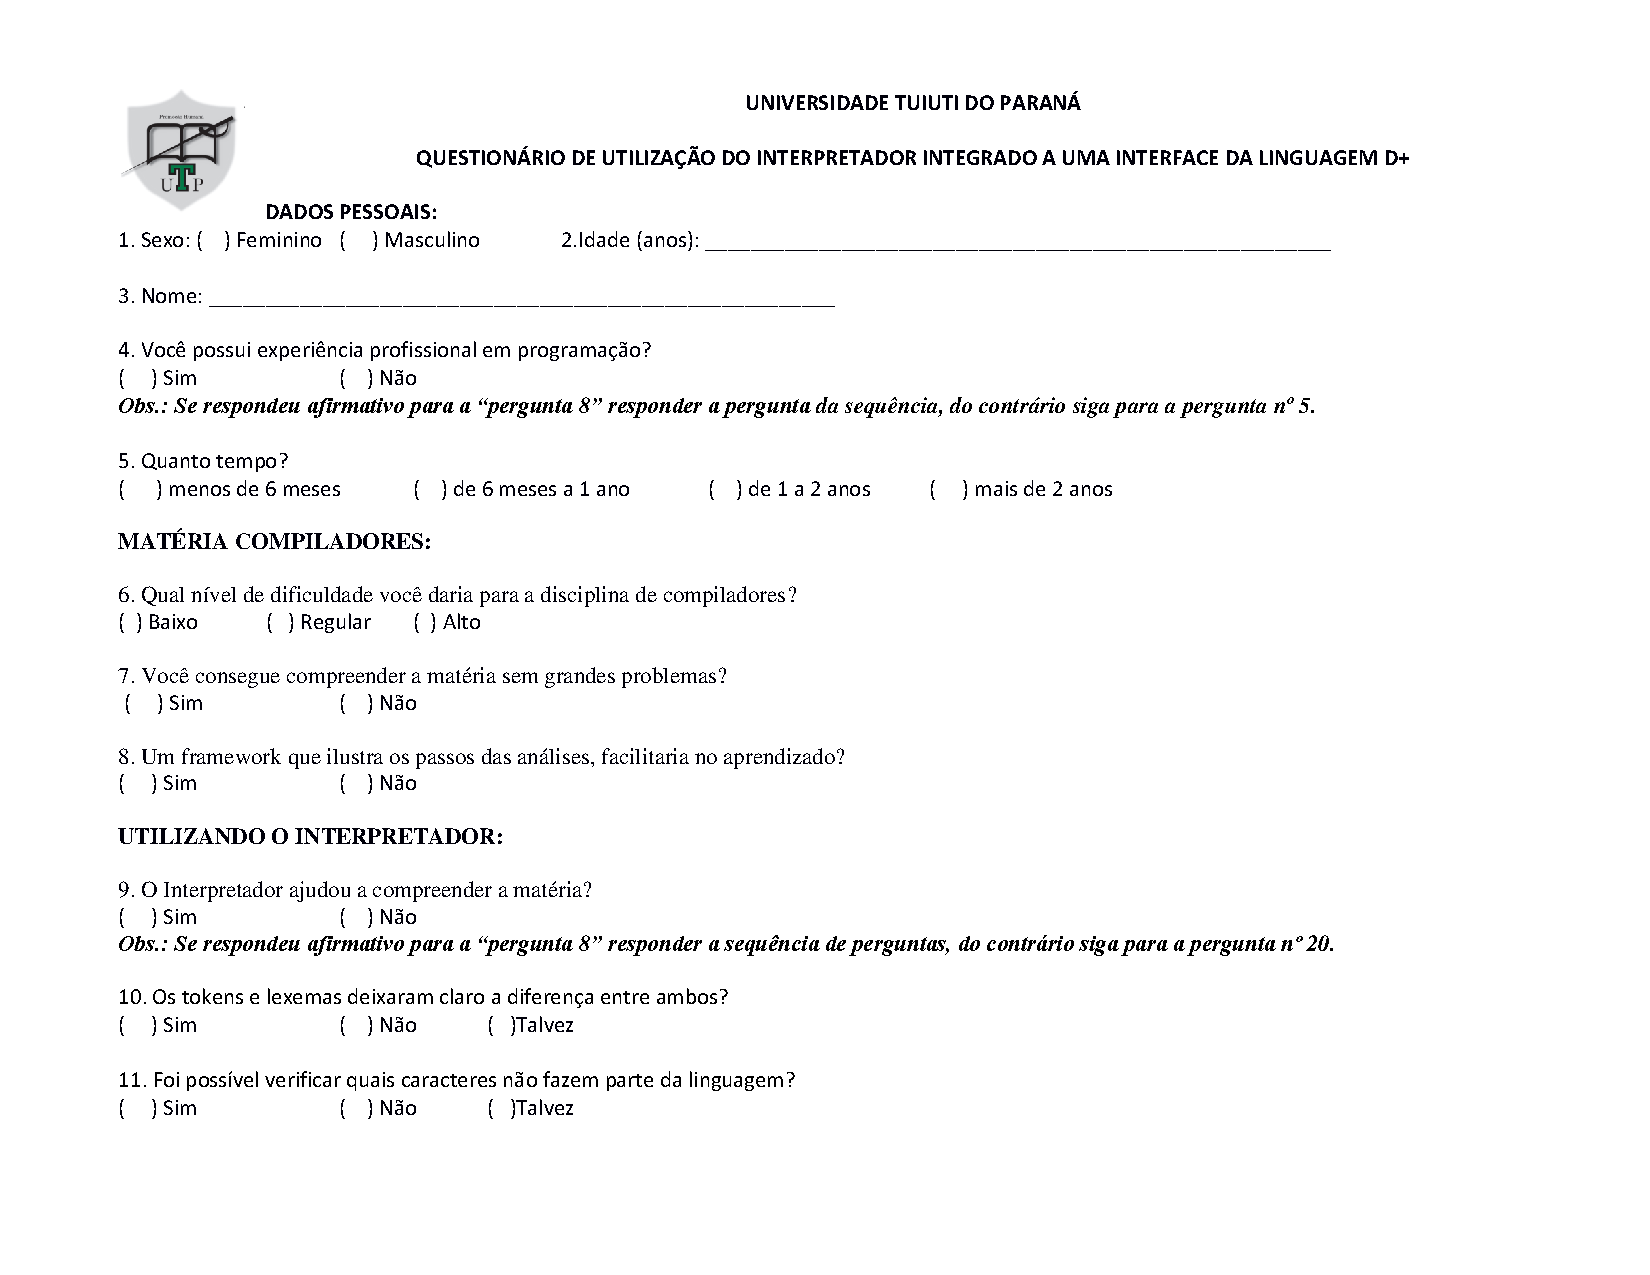
\includegraphics[scale=0.8, clip,trim=10mm 10mm 0mm 20mm, angle=-90, page=1]{QUESTIONARIO.pdf}

\includegraphics[scale=0.8, clip,trim=10mm 10mm 0mm 20mm, angle=-90, page=2]{QUESTIONARIO.pdf}

\includegraphics[scale=0.8, clip,trim=10mm 10mm 0mm 20mm, angle=-90, page=3]{QUESTIONARIO.pdf}

\apendice[apendice:automatos]{Autômatos Ativos}
\begin{figure}[htb]
    \legenda[fig:figura]{Autômato ativo estado 1}
    \fig{scale=1.0}{imagens/automatos/state1}
    \fonte{O próprio autor}
\end{figure}


\begin{figure}[htb]
    \legenda[fig:figura]{Autômato ativo estado 2}
    \fig{scale=0.7}{imagens/automatos/state2}
    \fonte{O próprio autor}
\end{figure}

\begin{figure}[htb]
    \legenda[fig:figura]{Autômato ativo estado 3}
    \fig{scale=0.8}{imagens/automatos/state3}
    \fonte{O próprio autor}
\end{figure}

\begin{figure}[htb]
    \legenda[fig:figura]{Autômato ativo estado 4}
    \fig{scale=0.8}{imagens/automatos/state4}
    \fonte{O próprio autor}
\end{figure}

\begin{figure}[htb]
    \legenda[fig:figura]{Autômato ativo estado 5}
    \fig{scale=0.6}{imagens/automatos/state5}
    \fonte{O próprio autor}
\end{figure}

\begin{figure}[htb]
    \legenda[fig:figura]{Autômato ativo estado 6}
    \fig{scale=0.6}{imagens/automatos/state6}
    \fonte{O próprio autor}
\end{figure}

\begin{figure}[htb]
    \legenda[fig:figura]{Autômato ativo estado 7}
    \fig{scale=0.6}{imagens/automatos/state7}
    \fonte{O próprio autor}
\end{figure}

\begin{figure}[htb]
    \legenda[fig:figura]{Autômato ativo estado 8}
    \fig{scale=0.6}{imagens/automatos/state8}
    \fonte{O próprio autor}
\end{figure}

\begin{figure}[htb]
    \legenda[fig:figura]{Autômato ativo estado 9}
    \fig{scale=0.6}{imagens/automatos/state9}
    \fonte{O próprio autor}
\end{figure}

\begin{figure}[htb]
    \legenda[fig:figura]{Autômato ativo estado 10}
    \fig{scale=0.6}{imagens/automatos/state10}
    \fonte{O próprio autor}
\end{figure}

\begin{figure}[htb]
    \legenda[fig:figura]{Autômato ativo estado 11}
    \fig{scale=0.6}{imagens/automatos/state11}
    \fonte{O próprio autor}
\end{figure}

\begin{figure}[htb]
    \legenda[fig:figura]{Autômato ativo estado 12}
    \fig{scale=0.6}{imagens/automatos/state12}
    \fonte{O próprio autor}
\end{figure}

\begin{figure}[htb]
    \legenda[fig:figura]{Autômato ativo estado 13}
    \fig{scale=0.6}{imagens/automatos/state13}
    \fonte{O próprio autor}
\end{figure}

\begin{figure}[htb]
    \legenda[fig:figura]{Autômato ativo estado 14}
    \fig{scale=0.6}{imagens/automatos/state14}
    \fonte{O próprio autor}
\end{figure}

\begin{figure}[htb]
    \legenda[fig:figura]{Autômato ativo estado 15}
    \fig{scale=0.6}{imagens/automatos/state15}
    \fonte{O próprio autor}
\end{figure}


\apendice[apendice:automatos]{Autômatos Desabilitados}
\begin{figure}[htb]
    \legenda[fig:figura]{Autômato desabilitado estado 1}
    \fig{scale=1.0}{imagens/automatos/stateDisabled1}
    \fonte{O próprio autor}
\end{figure}


\begin{figure}[htb]
    \legenda[fig:figura]{Autômato desabilitado estado 2}
    \fig{scale=0.7}{imagens/automatos/stateDisabled2}
    \fonte{O próprio autor}
\end{figure}

\begin{figure}[htb]
    \legenda[fig:figura]{Autômato desabilitado estado 3}
    \fig{scale=0.8}{imagens/automatos/stateDisabled3}
    \fonte{O próprio autor}
\end{figure}

\begin{figure}[htb]
    \legenda[fig:figura]{Autômato desabilitado estado 4}
    \fig{scale=0.8}{imagens/automatos/stateDisabled4}
    \fonte{O próprio autor}
\end{figure}

\begin{figure}[htb]
    \legenda[fig:figura]{Autômato desabilitado estado 5}
    \fig{scale=0.6}{imagens/automatos/stateDisabled5}
    \fonte{O próprio autor}
\end{figure}

\begin{figure}[htb]
    \legenda[fig:figura]{Autômato desabilitado estado 6}
    \fig{scale=0.6}{imagens/automatos/stateDisabled6}
    \fonte{O próprio autor}
\end{figure}

\begin{figure}[htb]
    \legenda[fig:figura]{Autômato desabilitado estado 7}
    \fig{scale=0.6}{imagens/automatos/stateDisabled7}
    \fonte{O próprio autor}
\end{figure}

\begin{figure}[htb]
    \legenda[fig:figura]{Autômato desabilitado estado 8}
    \fig{scale=0.6}{imagens/automatos/stateDisabled8}
    \fonte{O próprio autor}
\end{figure}

\begin{figure}[htb]
    \legenda[fig:figura]{Autômato desabilitado estado 9}
    \fig{scale=0.6}{imagens/automatos/stateDisabled9}
    \fonte{O próprio autor}
\end{figure}

\begin{figure}[htb]
    \legenda[fig:figura]{Autômato desabilitado estado 10}
    \fig{scale=0.6}{imagens/automatos/stateDisabled10}
    \fonte{O próprio autor}
\end{figure}

\begin{figure}[htb]
    \legenda[fig:figura]{Autômato desabilitado estado 11}
    \fig{scale=0.6}{imagens/automatos/stateDisabled11}
    \fonte{O próprio autor}
\end{figure}

\begin{figure}[htb]
    \legenda[fig:figura]{Autômato desabilitado estado 12}
    \fig{scale=0.6}{imagens/automatos/stateDisabled12}
    \fonte{O próprio autor}
\end{figure}

\begin{figure}[htb]
    \legenda[fig:figura]{Autômato desabilitado estado 13}
    \fig{scale=0.6}{imagens/automatos/stateDisabled13}
    \fonte{O próprio autor}
\end{figure}

\begin{figure}[htb]
    \legenda[fig:figura]{Autômato desabilitado estado 14}
    \fig{scale=0.6}{imagens/automatos/stateDisabled14}
    \fonte{O próprio autor}
\end{figure}

\begin{figure}[htb]
    \legenda[fig:figura]{Autômato desabilitado estado 15}
    \fig{scale=0.6}{imagens/automatos/stateDisabled15}
    \fonte{O próprio autor}
\end{figure}

\apendice[apendice:automatos]{Dados obtidos}
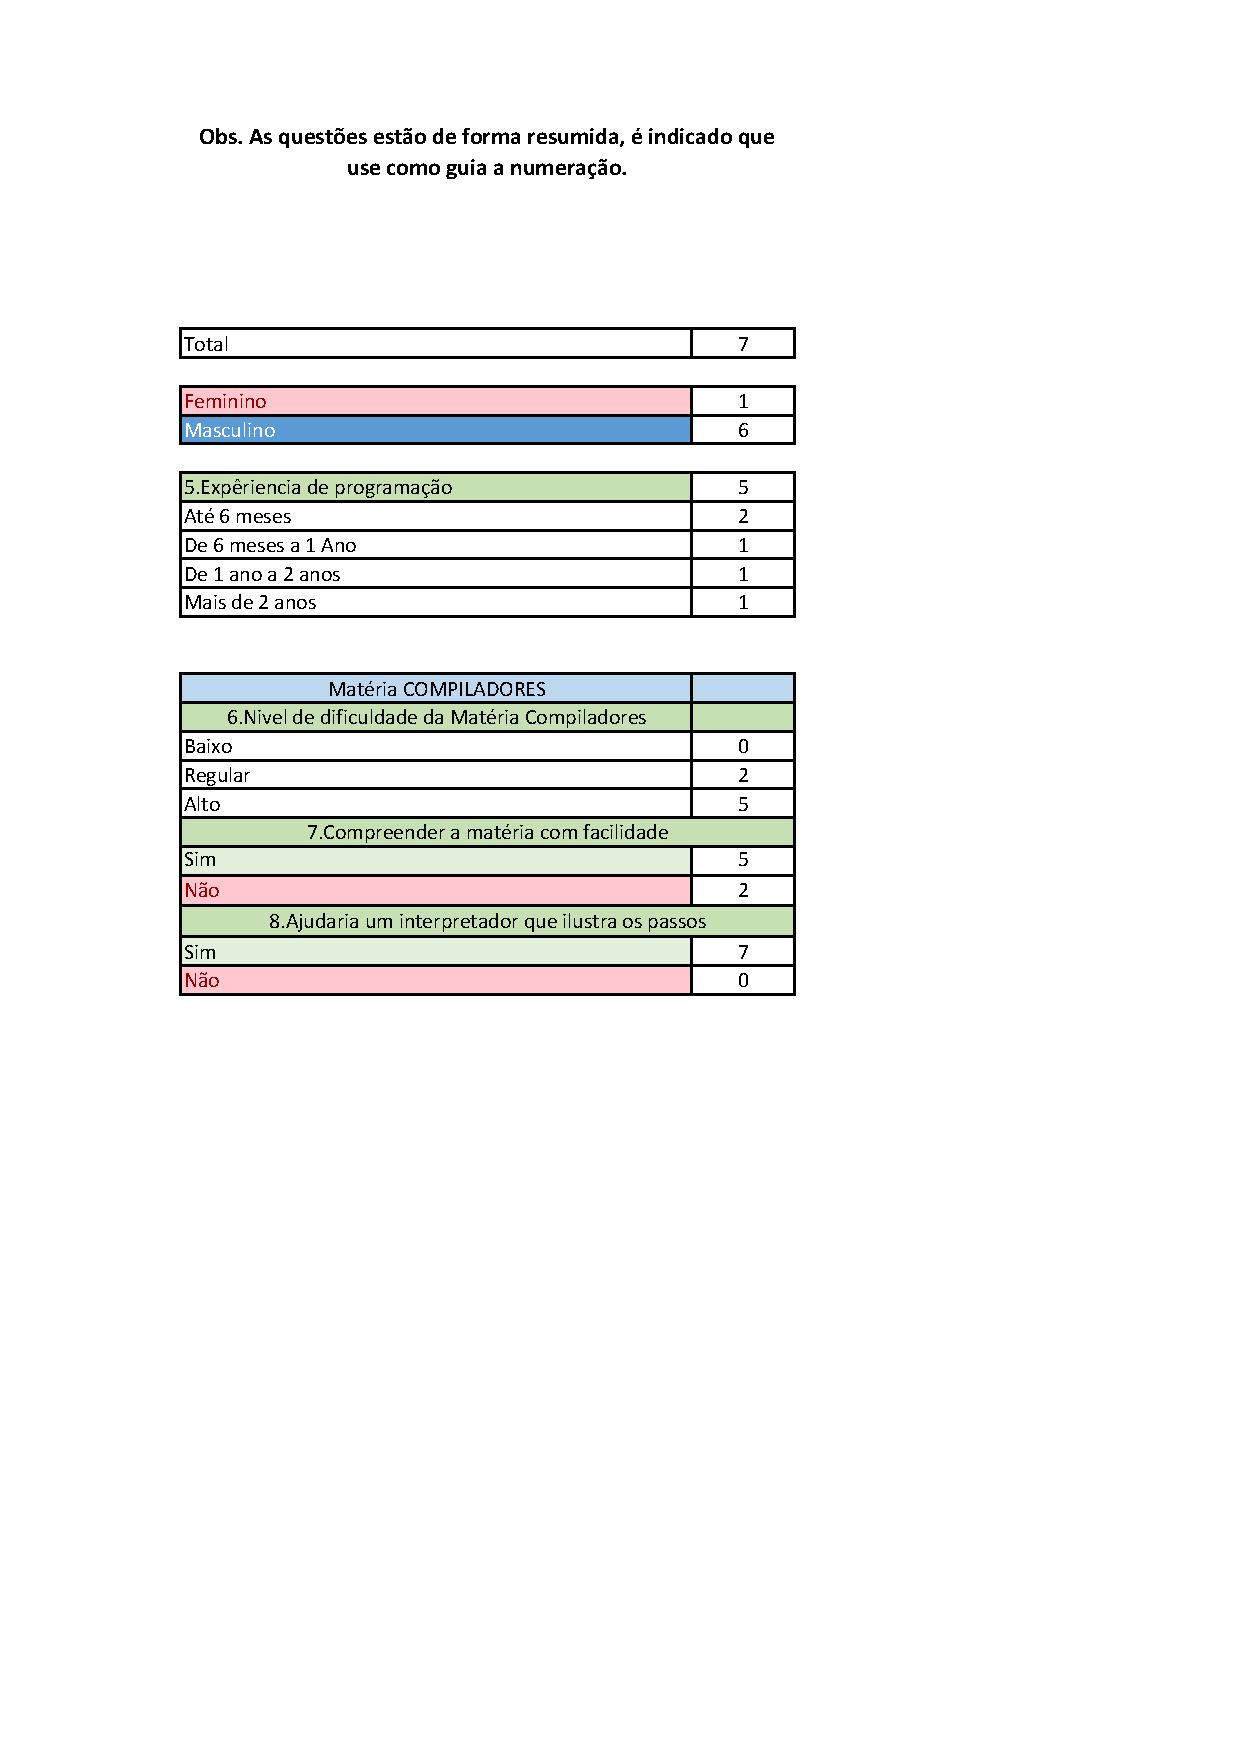
\includegraphics[scale=1.0, clip,trim=20mm 60mm 50mm 50mm, page=1]{resultado.pdf}

\includegraphics[scale=1.0, clip,trim=20mm 10mm 40mm 30mm, page=2]{resultado.pdf}

\includegraphics[scale=1.0, clip,trim=20mm 10mm 40mm 30mm, page=3]{resultado.pdf}

\includegraphics[scale=1.0, clip,trim=20mm 10mm 40mm 20mm, page=4]{resultado.pdf}

\apendice[apendice:codigoexemplo]{Códigos de Exemplo}

As figuras 78, 79, 80, 81 são exemplos de códigos da gramática D+.

\begin{figure}[htb]
    \legenda[fig:figura]{Código 1 da gramática D+}
    \fig{scale=1.5}{imagens/codigoparateste1}
    \fonte{O próprio autor}
\end{figure}

\begin{figure}[htb]
    \legenda[fig:figura]{Código 2 da gramática D+}
    \fig{scale=1.5}{imagens/codigoparateste2}
    \fonte{O próprio autor}
\end{figure}

\begin{figure}[htb]
    \legenda[fig:figura]{Código 3 da gramática D+}
    \fig{scale=1.5}{imagens/codigoparateste3}
    \fonte{O próprio autor}
\end{figure}

\begin{figure}[htb]
    \legenda[fig:figura]{Código 4 da gramática D+}
    \fig{scale=1.5}{imagens/codigoparateste4}
    \fonte{O próprio autor}
\end{figure}

\apendice[apendice:instalacao]{Instalação do Interpretador D+}

Para facilitar o acesso a esta framework, foi efetuado um deploy do interpretador D+ e criado um arquivo executável para efetuar a instalação do software, assim não precisando instalar o QtCreator e suas bibliotecas.

Para instalar o Interpretador execute o arquivo "InterpretadorD+", após executa ló, aparecera uma janela igual a figura 82, clique em next.

\begin{figure}[!htb]
    \legenda[fig:figura]{Janela de instalação 1}
    \fig{scale=1.0}{imagens/instalação1}
    \fonte{O próprio autor}
\end{figure}

A janela prosseguira e aparecera o local que você deseja instalar o software, selecione o local e clique em next, conforma e figura 83.

\begin{figure}[H]
    \legenda[fig:figura]{Janela de instalação 2}
    \fig{scale=1.0}{imagens/instalação2}
    \fonte{O próprio autor}
\end{figure}

Após prosseguir carregará uma pagina igual à figura 84, selecione o "Interpretador\_D+" e clique em next.

\begin{figure}[H]
    \legenda[fig:figura]{Janela de instalação 3}
    \fig{scale=1.0}{imagens/instalação3}
    \fonte{O próprio autor}
\end{figure}

A janela prosseguira e carregará uma janela igual à figura 85, clique em next.

\begin{figure}[H]
    \legenda[fig:figura]{Janela de instalação 4}
    \fig{scale=1.0}{imagens/instalação4}
    \fonte{O próprio autor}
\end{figure}

Clique em "Install" conforme a figura 86.

\begin{figure}[H]
    \legenda[fig:figura]{Janela de instalação 5}
    \fig{scale=1.0}{imagens/instalação5}
    \fonte{O próprio autor}
\end{figure}

Após a instalação clique em "Finish" igual a figura 87, e o interpretador esta disponível no menu iniciar.

\begin{figure}[H]
    \legenda[fig:figura]{Janela de instalação 6}
    \fig{scale=1.0}{imagens/instalação6}
    \fonte{O próprio autor}
\end{figure}
% ----------------------------------------------------------
% Anexos
% ----------------------------------------------------------
% Material complementar nao preparado pelo autor
%\anexo[apendice:QUESTIONARIO.pdf]{QUESTIONÁRIO DE UTILIZAÇÃO DO INTERPRETADOR INTEGRADO A UMA INTERFACE DA LINGUAGEM D+ }



\end{document}
